\documentclass[]{spie}  %>>> use for US letter paper
%\documentclass[a4paper]{spie}  %>>> use this instead for A4 paper
%\documentclass[nocompress]{spie}  %>>> to avoid compression of citations

\renewcommand{\baselinestretch}{1.0} % Change to 1.65 for double spacing
\newcommand{\aap}{Astronomy \& Astrophysics}
\newcommand{\procspie}{Proc.\ SPIE}
\newcommand{\aspconf}{ASP Conf.\ Ser.}
\newcommand{\qjras}{QJRAS}

\newcommand{\ascl}[1]{\href{http://www.ascl.net/#1}{ascl:#1}}
\newcommand{\arxiv}[1]{\href{http://arxiv.org/abs/#1}{arXiv:#1}}

\usepackage{amsmath,amsfonts,amssymb}
\usepackage{graphicx}
\usepackage[colorlinks=true, allcolors=blue]{hyperref}

\title{Investigating interoperability of the LSST Data Management software stack with Astropy}
% Jenness, Bosch, Owen, Parejko, Sick, Swinbank, de Val-Boro et al
\author[a]{Tim Jenness}
\author[b]{James Bosch}
\author[c]{Russell Owen}
\author[c]{John Parejko}
\author[a]{Jonathan Sick}
\author[b]{John Swinbank}
\author[b]{Miguel de Val-Boro}

\affil[a]{LSST Project Management Office, Tucson, AZ, U.S.A.}
\affil[b]{Princeton University, Princeton, NJ, U.S.A.}
\affil[c]{University of Washington, Seattle, WA, U.S.A}

\authorinfo{Further author information: (Send correspondence to T.J.)\\T.J.: E-mail: tjenness@lsst.org}

% Option to view page numbers
\pagestyle{empty} % change to \pagestyle{plain} for page numbers
\setcounter{page}{301} % Set start page numbering at e.g. 301

\begin{document}
\maketitle

\begin{abstract}
  The Large Synoptic Survey Telescope (LSST) will be an 8.4\,m optical survey telescope sited in Chile and capable of imaging the entire sky twice a week.
  The data rate of approximately 15\,TB per night and the requirements to both issue alerts on transient sources within 60 seconds of observing and also to create annual data releases means that automated data management systems and data processing pipelines are a key deliverable of the LSST construction project.
  The LSST data management software has been in development since 2004 and, like other software developed in that era such as CASA, is based on a C++ core with a Python control layer.
  The software consists of nearly quarter of a million lines of code covering the system from fundamental WCS and table libraries to pipeline environments and distributed process execution.

  The Astropy project began in 2011 as an attempt to bring together disparate open source Python projects and build a core standard infrastructure that can be used by and built upon by the astronomy community.
  This project has been phenomenally successful in the years since it has begun and has grown to be the de facto standard for Python software in astronomy.
  Astropy brings with it considerable expectations from the community on how astronomy Python software should be developed and it is clear that by the time LSST is fully operational in the 2020s many of the prospective users of the LSST software stack will assume that Astropy software will be integrated.

  In this paper we describe the overlap between the LSST science pipeline software and Astropy software and investigate areas where the LSST software provides new functionality.
  We also discuss the possibilities of re-engineering the LSST science pipeline software to build upon Astropy, including the option of contributing affiliated packages.
\end{abstract}

% Include a list of keywords after the abstract
\keywords{Astronomy Software, Python, Code Reuse}

\section{INTRODUCTION}
\label{sec:intro}  % \label{} allows reference to this section

The Large Synoptic Survey Telescope (LSST)\cite{2008arXiv0805.2366I} will be an 8.4\,m optical survey telescope sited in Chile\cite{2014SPIE.9145E..1AG} and capable of imaging the entire sky twice a week.
The data rate of approximately 15\,TB per night\footnote{See \url{http://lsst.org/scientists/keynumbers} for additional numbers.} and the requirements to both issue alerts on transient sources within 60 seconds of observing and also to create annual data releases means that automated data management systems and data processing pipelines are a key deliverable of the LSST construction project\cite{2016_adassxxv_O3-1}.

The difficulty of sharing code between telescopes has long been a topic of discussion in the astronomy software community\cite{1998ASPC..145..142M,1999ASPC..172...11E,2001ASSL..266..163S,2002SPIE.4844..321E}.
Historically there have been some successes in fundamental libraries, such as SOFA\cite{2011SchpJ...611404H}, CFITSIO\cite{1999ASPC..172..487P} and wcslib\cite{2011ascl.soft08003C}, and in environments, such as IRAF\cite{1986SPIE..627..733T}, AIPS\cite{1996ASPC..101...37V} and Starlink\cite{1982QJRAS..23..485D}.
Despite these, there is still a tendency for a new project to embark on the creation of a new environment or software infrastructure if there are slight requirements mismatches and no external political will to adopt a specific software suite.
The growth in the Open Source software movement\cite{2006OpenSources} and recent explosion in support tools such as git and GitHub for code sharing\cite{2014IACWSLima}, makes the process of software reuse far easier than it has ever been.

The LSST data processing pipeline software has been in development since 2004\cite{2004AAS...20510811A,2010SPIE.7740E..15A,2016_adassxxv_P056} and during these 16 years of development much has changed in the Python, C++ and astronomy software world.


\section{The LSST Science Pipeline Software}

As with other software developed in the early 2000s, such as CASA\cite{2012ASPC..461..849P}, the LSST science pipeline software is based on a C++ core with a Python control layer.
The general layout of the code is shown in Fig.~\ref{fig:layers}.
In this paper we focus on the algorithmic and framework code provided by the \texttt{afw} and \texttt{meas\_} packages as these are the packages that have most in common with the Astropy core and affiliated packages.

\begin{figure} [ht]
\begin{center}
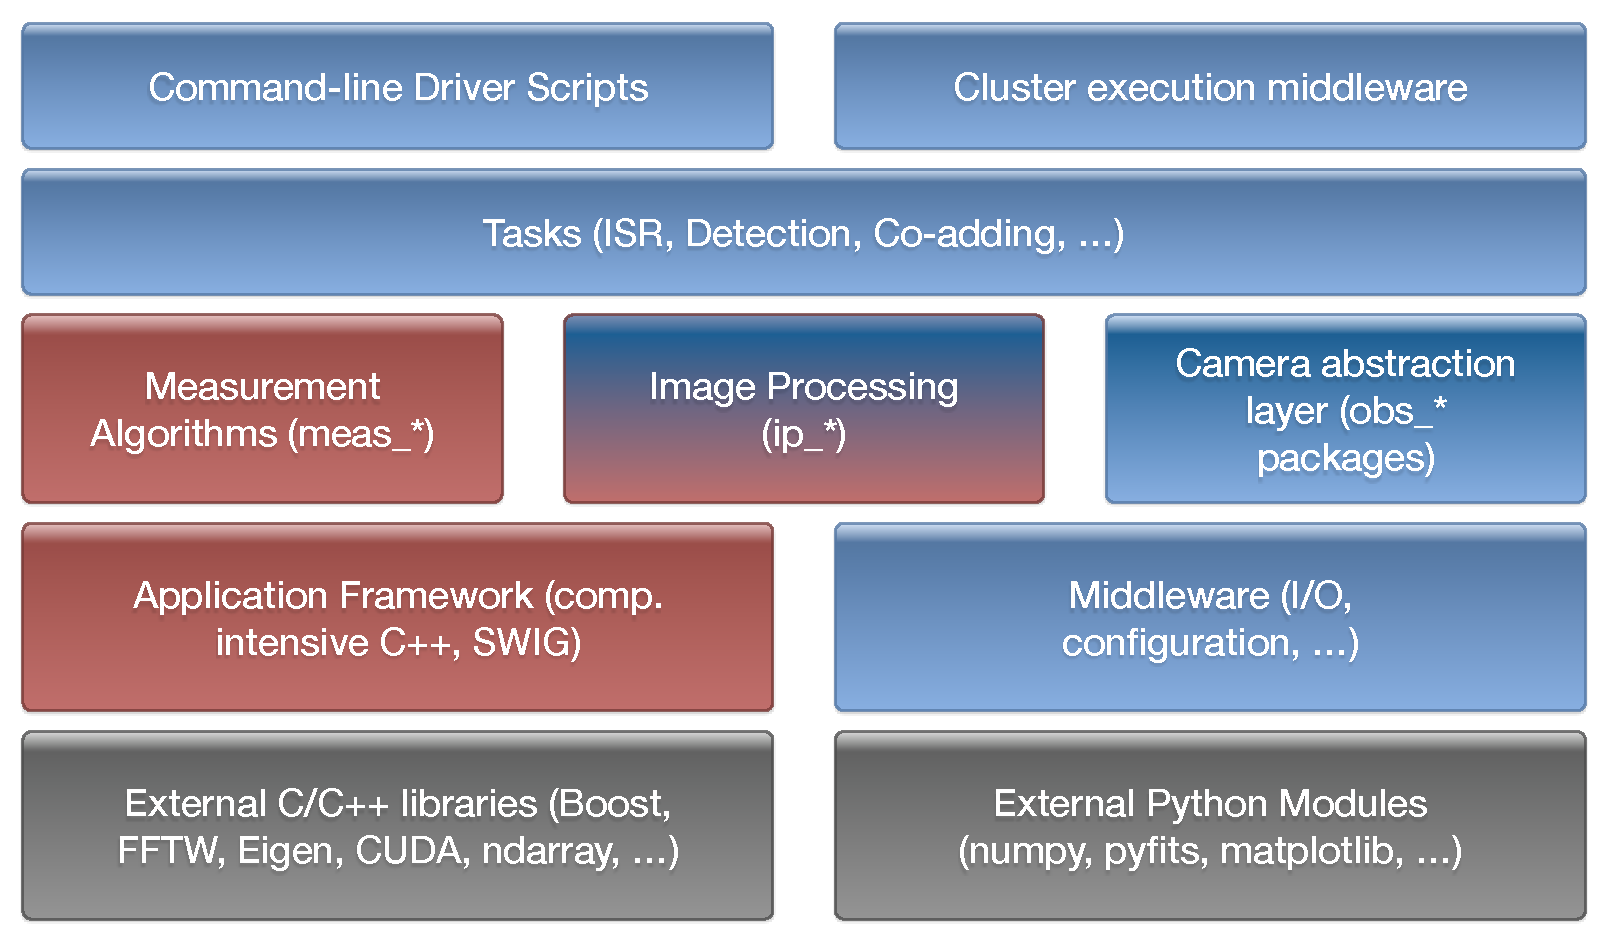
\includegraphics[height=5cm]{Software-Layers}
\end{center}
\caption[layers]
%>>>> use \label inside caption to get Fig. number with \ref{}
{\label{fig:layers}
Structure of the LSST data management software.
At the bottom there are external packages (black), on the lower left (red) are the computationally intensive packages that are mainly written in C++ with SWIG wrappers making the code available in Python, and the remainder (blue) are mostly Python.}
\end{figure}

\begin{figure} [ht]
\begin{center}
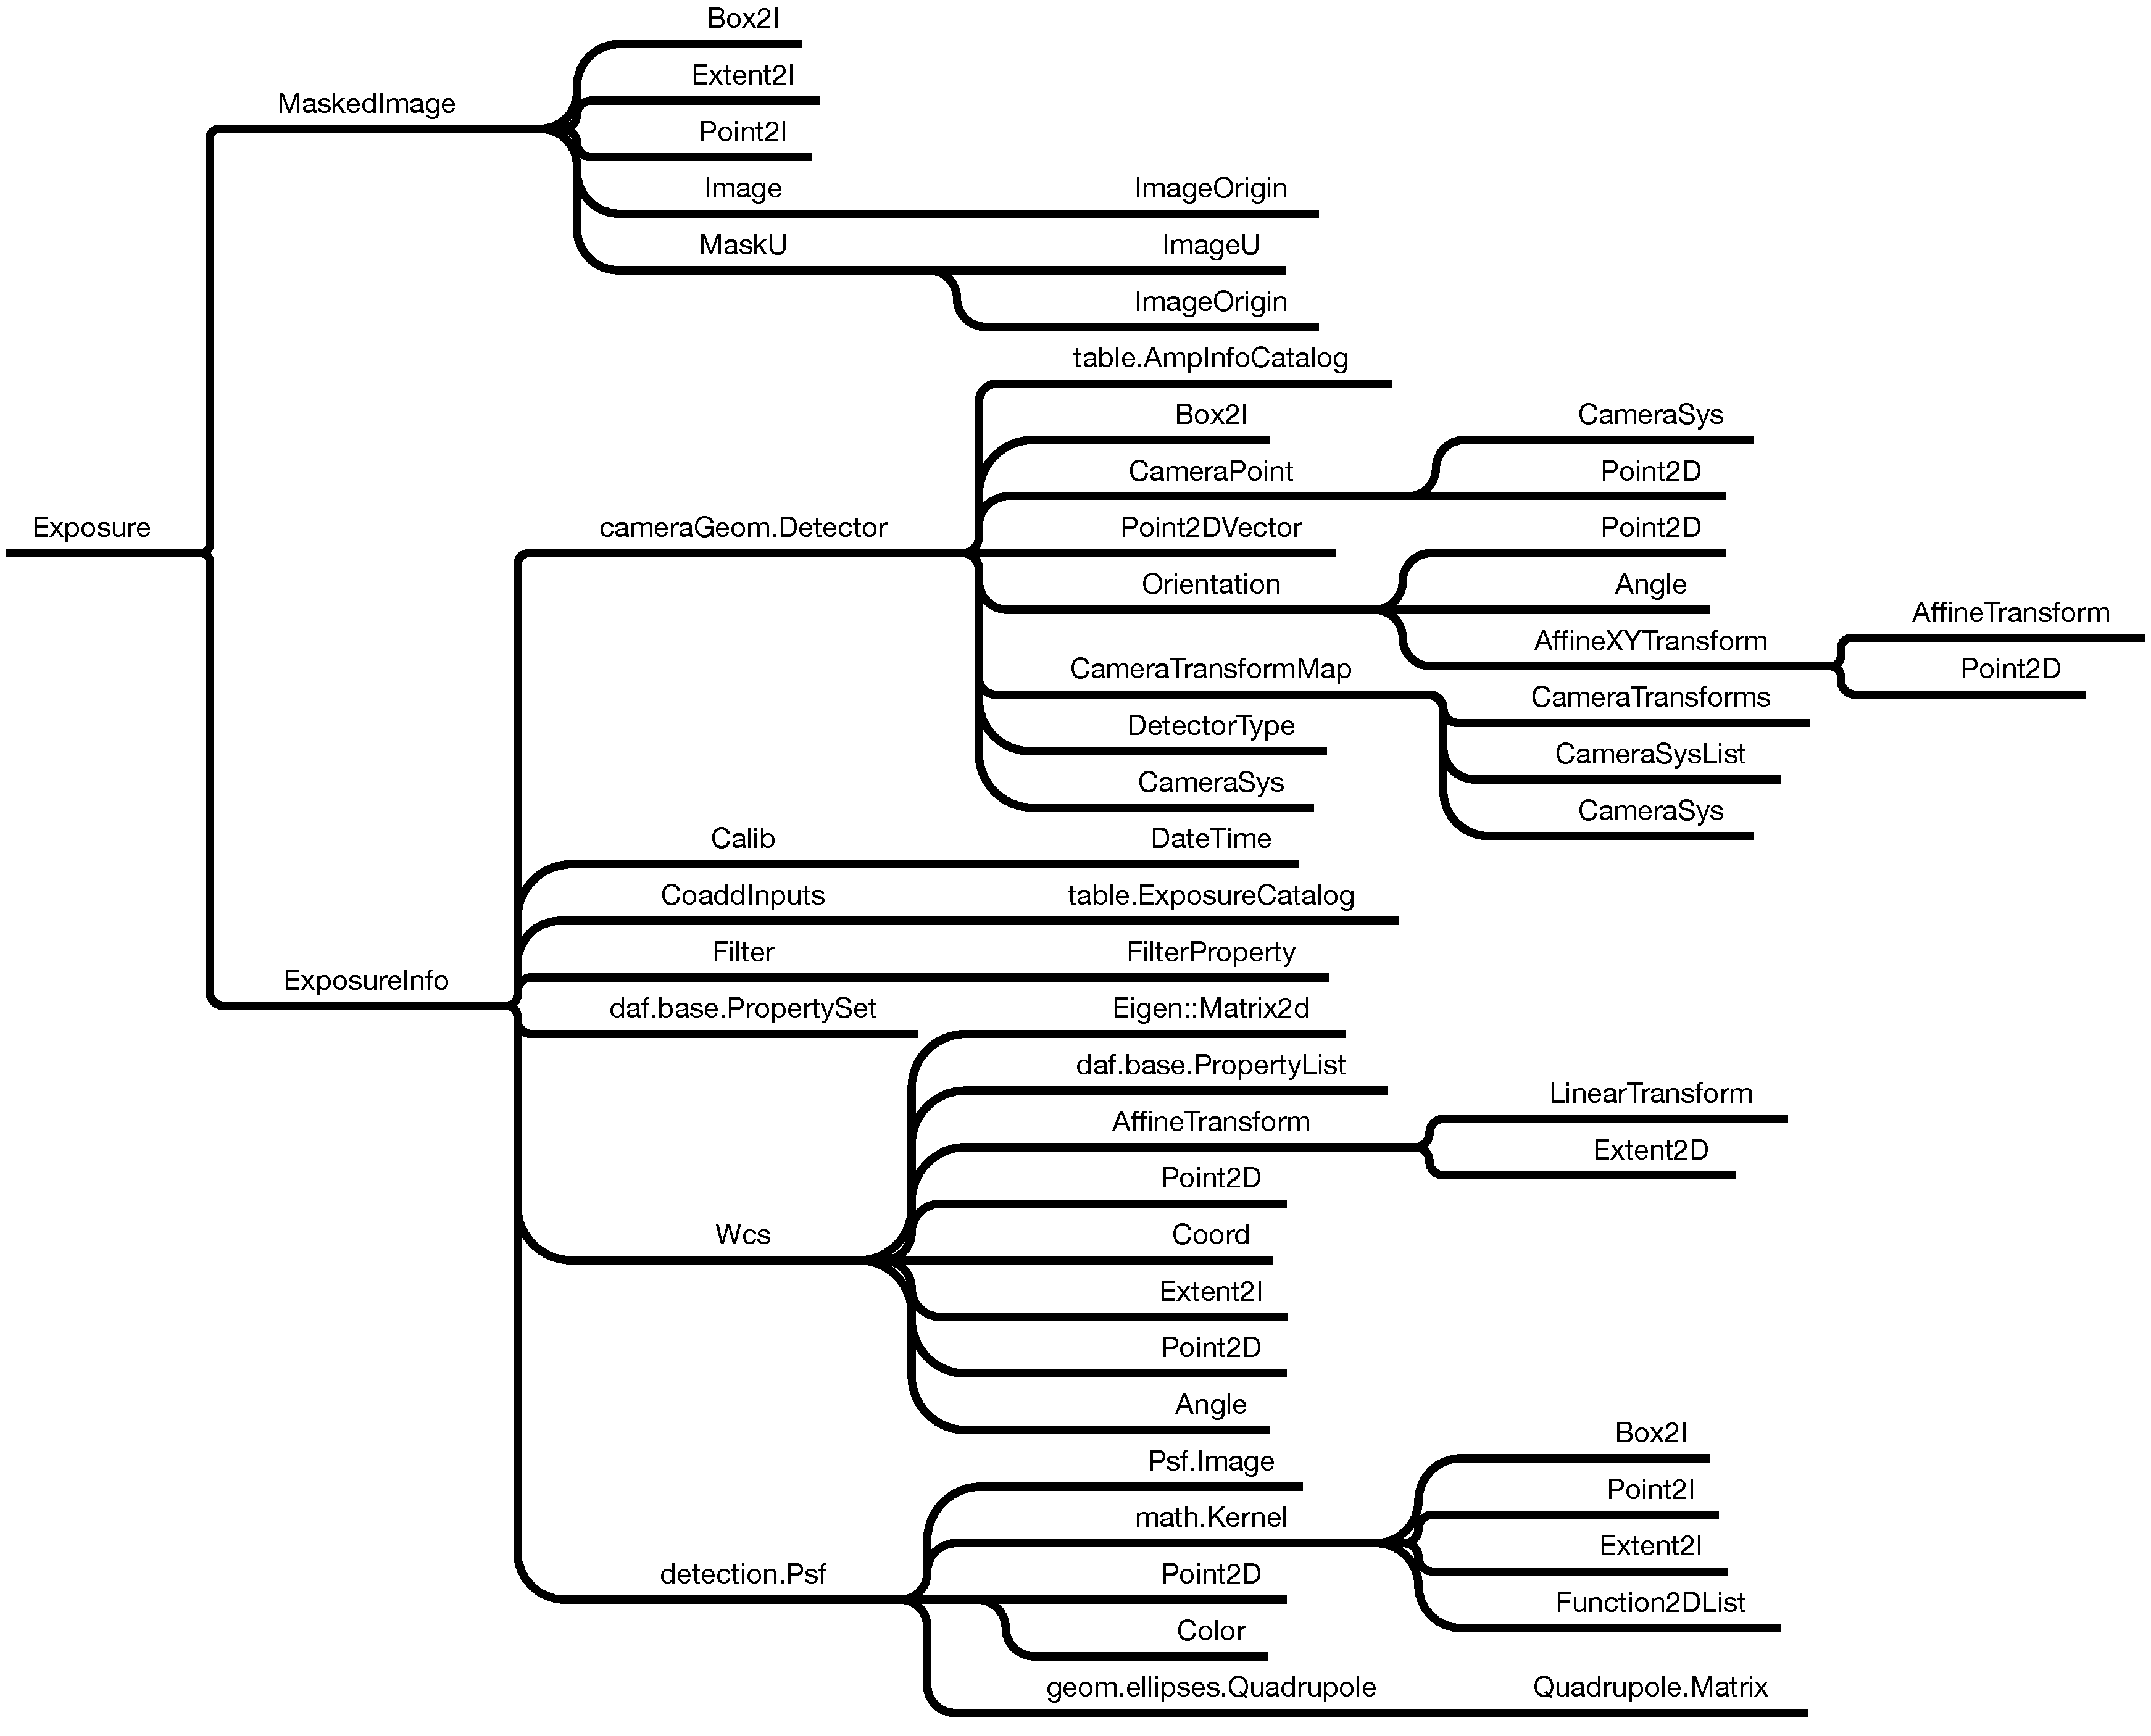
\includegraphics[width=\textwidth]{exposure-dependencies}
\end{center}
\caption[layers]
%>>>> use \label inside caption to get Fig. number with \ref{}
{\label{fig:exposure}
The classes that are used to define a \texttt{lsst.afw.image.ExposureX}.}
\end{figure}

\section{Astropy}

Python has become the de facto standard programming language for astronomy\cite{2000ASPC..216...59G,2006ASPC..351..343H,2006ASPC..351..497K,2011ASPC..442..425G,2012SPIE.8451E..02J} and is now the default choice for new projects and for teaching.
The Astropy\cite{2013A&A...558A..33A} project grew out of a support mailing list in 2011 to become a very successful hub for the development of Python packages for astronomy.
Astropy has two key concepts.
The first is to place generic astronomy code into the \emph{core} package that is brought in via \texttt{import astropy}; the second is to support and encourage the concept of \emph{affiliate} packages that are packages that use the \texttt{astropy} package and follow the same

\section{Synergies}

\section{Suggested modifications to LSST}

\subsection{Packaging}

The LSST data management software uses the EUPS tool\cite{EUPS} to manage versions and dependencies.
It is used to ensure that the versions of all packages used for a particular processing run can be assigned a single number and also to track the packages that were part of a single build.
Development versions can easily be included along with versions from builds done in the past.
This can significantly simplify debugging cycles and aid with provenance tracking but it is a complex environment with a steep learning curve and most users of LSST software outside of the data center and LSST developer community do not need this power.

LSST packages are built using the SCons tool\footnote{\url{http://www.scons.org}}\cite{2005Scons1377085}.
SCons is an alternative tool to Make and CMake that is written entirely in Python.
This allows developers to use Python for their library code and build system whilst making use of the powerful source code dependency tracking provided by SCons to prevent wasteful recompilation of files that have not been affected by local edits.

Unfortunately for SCons the majority of the Python community have adopted a simpler build system based around the convention of a \texttt{setup.py} file that can be executed to do the build.
This file uses \texttt{distuils} or \texttt{setuptools} to determine what should be built and can handle most cases where external C/C++ code should be compiled into the Python package.
There is a strong expectation that any packages made available to the Astropy community should follow the standard Python build convention of supporting \texttt{python setup.py build} and this is a requirement if we wish to make some LSST packages \emph{Astropy affiliated packages}.
This also allows packages to be distributed on the Python Package Index (PyPI\footnote{\url{https://pypi.python.org}}) providing the ability for a general user to use \texttt{pip install lsst\_apps} to install the LSST software.

As a proof of concept we have demonstrated that an LSST package using the standard LSST directory layout can be built using a \texttt{setuptools}.
EUPS is used to determine dependencies and this information can be converted to a standard \texttt{setuptools} dependency request.
To get this working on PyPI it is necessary either to generate the \texttt{setup.py} using a SCons target or else use EUPS directly in the \texttt{setup.py}.
The latter would require that EUPS is also available from PyPI (it currently is not) but might be less prone to errors.

\subsection{Astronomical Coordinates}

The LSST \texttt{afw.coord} package provides coordinate conversions between ICRS, FK5, Galactic, ecliptic and topocentric coordinate systems.
It is written in C++ and has no external dependencies on standard coordinate libraries.
The \texttt{astropy.coordinates} package provides a very usable Python API on top of the standard ERFA astrometry C library\footnote{ERFA is a relicensed version of the standard SOFA library\cite{SOFA}.}.
It supports all the coordinate systems provided by the LSST package and many more including FK4.

The LSST C++ code does not use any system other than ICRS therefore we are proposing to remove this package and replace it with a simple spherical coordinates class.
All the Python code will then be modified to use \texttt{astropy.coordinates} and at the Python/C++ boundary coordinates will be converted to/from ICRS.

\section{Tables}

LSST and Astropy both have table libraries, but these have different data models and hence different strengths.
LSST's are better for row-based access and provide a limited ORM layer that's valuable for pipeline use when the columns are known in advance and data are appended to the table, while Astropy's excel at column-based access and use in interactive analysis.
Furthermore, Astropy tables now support export to PANDAS data frames\cite{mckinney-proc-scipy-2010}, opening up a richer environment for query-based analysis.
We anticipate being able to do a lot by just creating AstroPy views to LSST table objects, thereby not doubling the memory requirements, and we have been able to put together a proof-of-concept implementation for doing this.

\section{Integration Options}

\section{Conclusions}

\acknowledgments\

This material is based upon work supported in part by the National Science Foundation through Cooperative Support Agreement (CSA) Award No.\ AST--1227061 under Governing Cooperative Agreement 1258333 managed by the Association of Universities for Research in Astronomy (AURA), and the Department of Energy under Contract No.\ DE--AC02--76SF00515 with the SLAC National Accelerator Laboratory.
Additional LSST funding comes from private donations, grants to universities, and in-kind support from LSSTC Institutional Members.

% References
\bibliography{lsst-astropy} % bibliography data in report.bib
\bibliographystyle{spiebib} % makes bibtex use spiebib.bst

\end{document}
